\insertdesignoverview{Drivetrain}
{Create a small, light drivetrain that can move quickly between the warehouse and both hubs and can fit in the gap between the barriers. Come up with a way to have more control with steering. Have several attachment points for easy integrations of new iterations of parts.
} % Goals of the mechanism
{10-12.JPG}% CAD Image
{drivetrain_1.JPG}% Build Image
{Medical Grade Polycarbonate, Nylon Plastic, Polyurethane Belts, 1/16” aluminum sheet metal}% Materials ex. 0.25" MDF, Aluminum, etc
{3D Printing, Brazing, Sheet Metal Shearing and Breaking}% Manufacturing Processes ex. Laser Cut, 3D print, etc.

\subsection*{How it Works}
To accomplish our goal of having greater control and speed when moving in between the warehouse and shipping hubs, we designed a very unique tricycle design that has one turning front wheel and two powered back wheels. Although it has only three wheels,  our drivetrain steers very similarly to how a car steers. The drivetrain is composed of two main sections: the main chassis and the front wheel module. The main chassis is a 9.5 by 8.5 inch monolithic 3D printed part made out of polycarbonate, a very strong type of plastic. This material combined with efficient design techniques like ribs and pocketing holes allowed for the creation of a light yet very strong drivetrain. This larger half of the drivetrain holds two 20:1 REV HD Hex motors which are connected to the back 2 wheels with pulleys and belts. The front wheel assembly is printed out of nylon and is attached to the front of the main chassis and holds the front wheel and its steering mechanism. Controlled by a servo connected to the light-up front wheel with a belt and pulley. To protect the front wheel, we used folded sheet metal to create an aluminum front bumper for the robot.

% \begin{figure}[htp]
% \centering
% 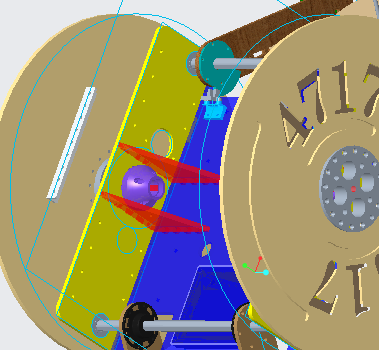
\includegraphics[width=.8\linewidth]{Design_Overview/DT_cad.PNG}
% \caption{Another look at the CAD of our Drivetrain}
% \label{fig:iteration}
% \end{figure}

\subsection*{Iterations}
At the beginning of the season, we tried using a small tank drivetrain. Tank drive, though a well established FTC standard, had a hard time making the arc shaped paths that are required to move from the warehouse to the shipping hubs. After coming up with the tricycle design, we designed and tested it, finding that it had much greater control and speed while navigating through the gaps than the tank drive did.

%PUT THESE PHOTOS HERE 
% Image: Design_Drivetrain_LaserRange1
% Design_Drivetrain_LaserRange2


In addition, we have developed an algorithm called the “Software Differential” which takes the value of steering wheel angle as a parameter and automatically modifies the velocities of the back wheels to be able to accurately follow a curve. Pictures of the derived math equations are shown below.


\subsection*{Mechanism Accomplishments}
\begin{itemize}
    \item Fits between the barrier
    \item Lightweight while strong design
    \item More control when driving than past drive trains
    \item Maintains fast speeds
\end{itemize} 

